\documentclass{standalone}
\usepackage{tikz}
\usetikzlibrary{patterns, angles}

\begin{document}
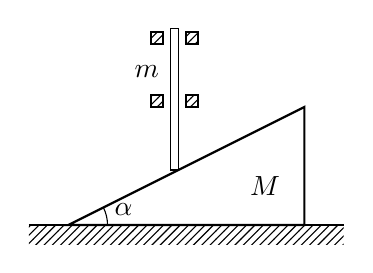
\begin{tikzpicture}
	\coordinate (A) at (0.5, 0);
    \coordinate (B) at (3.5, 0);
    \coordinate (C) at (3.5, 1.5);
       
	\draw [draw=none, pattern=north east lines] (0,-0.25) rectangle (4, 0);	
	\draw [thick] (0, 0) -- (4, 0);

	\draw [draw=none, pattern=north east lines] (2,1.5) rectangle (2.15, 1.65);	
	\draw [thick] (2,1.5) -- (2, 1.65) -- (2.15, 1.65) -- (2.15,1.5) -- cycle;

	\draw [draw=none, pattern=north east lines] (1.7,1.5) rectangle (1.55, 1.65);	
	\draw [thick] (1.7,1.5) -- (1.7, 1.65) -- (1.55, 1.65) -- (1.55,1.5) -- cycle;

	\draw [draw=none, pattern=north east lines] (1.7,2.3) rectangle (1.55, 2.45);	
	\draw [thick] (1.7,2.3) -- (1.7, 2.45) -- (1.55, 2.45) -- (1.55,2.3) -- cycle;

	\draw [draw=none, pattern=north east lines] (2,2.3) rectangle (2.15, 2.45);	
	\draw [thick] (2,2.3) -- (2, 2.45) -- (2.15, 2.45) -- (2.15,2.3) -- cycle;

	\draw [thick] (A) -- (B) -- (C) -- cycle;
	\draw (1.9,0.7) -- (1.9, 2.5) -- (1.8, 2.5) -- (1.8,0.7) -- cycle;	
	
	\node at (3,0.5) {$M$};
	\node at (1.5,1.95) {$m$};
	\pic [draw, -, angle eccentricity=1.5] {angle = B--A--C};
	\node [right=20pt, above] at (A) {$\alpha$};
\end{tikzpicture}
\end{document}